\documentclass[pdf]{beamer}
\usepackage[latin1]{inputenc}
\usepackage{multirow}
\usetheme{Berkeley} %Warsaw
\usecolortheme{wolverine}


\begin{document}

\title[GWAS]{Genome Wide Assocation Studies (GWAS)}
\subtitle{BCB 504: Applied Bioinformatics\\}
\author[Matt Settles]{Matt Settles}
\institute{University of Idaho\\ Bioinformatics and Computational Biology Program}
\date{\today}


%% Title page
\begin{frame}[plain]
  \titlepage
\end{frame}


%% Outline
\begin{frame}[plain] 
  \frametitle{Outline}
  \tableofcontents
\end{frame}

\section{Illumina Genotyping}
\begin{frame}
  \frametitle{Illumina Genotyping}
  Illumina's genotype technology uses \alert{Tag SNPs} to genotype millions of markers simultaneously. A tag SNP is a representative single nucleotide polymorphism (SNP) in a region of the genome with high linkage disequilibrium (the non-random association of alleles at two or more loci). It is possible to identify genetic variation without genotyping every SNP in a chromosomal region.
  \begin{center}
    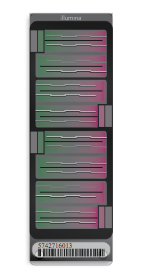
\includegraphics[scale=0.3]{Figures/omni.png} 
    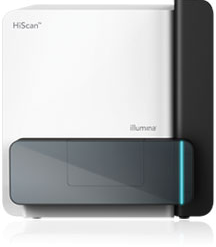
\includegraphics[scale=0.3]{Figures/hiscan.png} 
  \end{center}
  \begin{center}
       \href{http://www.illumina.com/applications/gwas.ilmn}{Illumina Genotyping}
  \end{center}  
\end{frame}

\begin{frame}
  \frametitle{Chips}
  \begin{center}
  Omni Whole-Genome Arrays
  \begin{tabular}{lcc}
\hline 
BeadChip & Array Format & Markers per Sample \\ 
\hline
HumanOmni5-Quad & 4 & \string~ 4.3 million \\ 
HumanOmni2.5S & 8 & \string~ 2.5 million \\ 
HumanOmni2.8-8 & 8 & \string~ 2.5 million \\ 
HumanOmni1S & 8 & \string~ 1.25 million \\ 
HumanOmni1-Quad & 4 & \string~ 1.1 million \\ 
HumanOmniExpress & 12 & \string~ 700,000 \\ 
HumanCytoSNP-12 & 12 & \string~ 300,000 \\ 
\hline 
\end{tabular} 
\end{center}  
\alert{Species:} Human, Mouse, Rat, Bovine, Equine, Porcine, Ovine, Canine
\end{frame}

\section{Preprocessing of Data}
\begin{frame}
\frametitle{Preprocessing of Data}
Data begins as intensity values for each sample and each snp (2-color, one for each candidate allele).\\
Data is then:
\begin{itemize}
  \item normalized
  \item converted to polor coordinates
  \item genotype clusters are generated
  \item GenCall score is calculated
  \item final genotype is determined
\end{itemize}
\end{frame}

\begin{frame}
\frametitle{Cartesian and Polar Coordinates}
\begin{description}
\item[Cartesian] coordinates use the X-axis to represent the intensity of the A allele and the Y-axis to represent the intensity of the B allele.
\item[Polar] coordinates use the X-axis to represent normalized theta (the angle deviation from pure A signal, where 0 represents pure A signal and 1.0 represents pure B signal), and the Y-axis to represent the distance of the point to the origin (normalized R).
\end{description}
\alert{For the Radius (R), the Manhattan distance ($A+B$) is used rather than the Euclidian distance ($sqrt(A*A+B*B)$).}
\end{frame}

\begin{frame}
\frametitle{Cartesian and Polar Coordinates}
\begin{center}
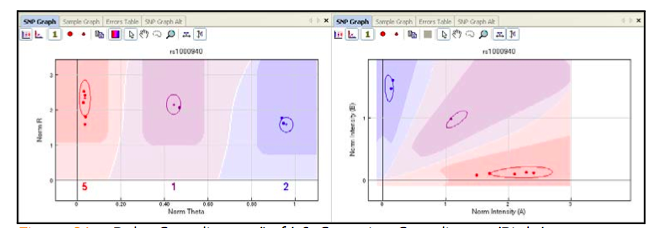
\includegraphics[scale=0.45]{Figures/car_polar.png} 
\end{center}
\end{frame}

\begin{frame}
\frametitle{Clustering}
Given a population of samples that exhibit three genotypes for every SNP, a clustering algorithm is used to determine the cluster positions of the genotypes. If certain SNPs have one or two clusters that lack representation, the algorithm will estimate the missing cluster positions.\\
\vspace{0.2in}
The lower the minor allele frequency, the more samples are required to achieve representation of all clusters. A population of 100 or more samples is typically recommended.
\vspace{0.2in}
The cluster ovals represent the location of the clusters with two standard deviations.
\end{frame}

\begin{frame}
\frametitle{Clusters}
\begin{center}
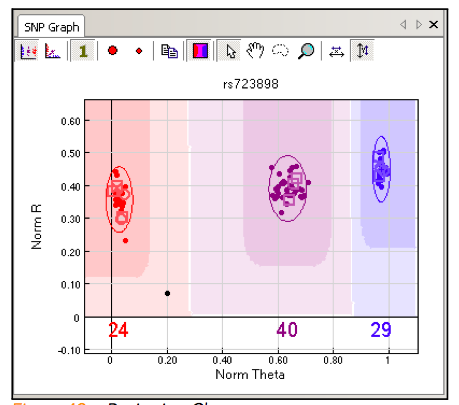
\includegraphics[scale=0.5]{Figures/Clusters.png} 
\end{center}
\end{frame}


\begin{frame}[allowframebreaks]
\frametitle{GenCall Score}
GenCall Score is a quality metric that indicates the reliability of each genotype call. The GenCall Score is a value between 0 and 1 assigned to every called genotype. Genotypes with lower GenCall scores are located further from the center of a cluster and have a lower reliability.\\
GenCall Scores are calculated using information from the clustering of the samples. To get a GenCall Score, each SNP is evaluated based on the following characteristics of the clusters:
\begin{itemize}
  \item angle
  \item dispersion overlap
  \item intensity
\end{itemize}
There is no global interpretation of a GenCall Score, as the score depends on the clustering of your samples at each SNP, which is affected by many different variables including the quality of the samples and the loci.\\
\vspace{0.2in}
Final genotype for a sample and SNP pair is then the cluster the sample resides in a whether the sample meets the GenCall Score cutoff.\\
Illumina recommends that you use a GenCall Score cutoff of 0.15 for Infinium products and 0.25 for GoldenGate products.\\
\end{frame}

\subsection{Data format}
\begin{frame}[fragile]
  \frametitle{Data Format}
\begin{tiny}
\begin{verbatim}
[Header]
GSGT Version	1.9.4
Processing Date	2/13/2012 12:06 AM
Content		BovineHD_B.bpm
Num SNPs	777962
Total SNPs	777962
Num Samples	1588
Total Samples	1588
[Data]
SNP Name	Sample ID	Allele1-Forward	Allele2-Forward	Allele1-Top	Allele2-Top	
Allele1-AB	Allele2-AB	GC Score	X	Y
ARS-BFGL-NGS-106614	2891	C	C	C	C	B	B	0.4913	0.041	1.125
ARS-BFGL-NGS-89367	2891	T	G	A	C	A	B	0.8079	0.757	0.661
BovineHD3100000001	2891	T	T	A	A	A	A	0.4954	1.297	0.052
BovineHD3100000002	2891	A	A	A	A	A	A	0.9381	1.225	0.022
BovineHD3100000003	2891	C	C	G	G	B	B	0.4787	0.012	0.669
\end{verbatim}
\end{tiny}
\end{frame}

\section{Data Cleaning}
\begin{frame}
\frametitle{Cleaning the data}
Sample cleaning
\begin{itemize}
  \item missing genotypes (ie greater than 10\%)
  \item if parents were also genotyped, mendelian inheritance 
  \item Excessive autosomal homozygosity
  \item Sex misassignment (X heterozygosity)
\end{itemize}
Marker cleaning
\begin{itemize}
\item Minor allele frequency (MAF) $<0.01$
\item Missing values (ie $>5$\%)
\item Hardy Weinberg expectation (p-value $< 10^{-7}$ in founders)
\end{itemize}
\end{frame}  

\begin{frame}
\frametitle{Batch QA}
Check for batch effects
\begin{itemize}
\item MAF by batch
\item MAF by plate
\item MAF by sample type 
\end{itemize}
\end{frame}

\section{software}
\begin{frame}
\frametitle{software}
PLINK\\
\href{http://pngu.mgh.harvard.edu/~purcell/plink/}{http://pngu.mgh.harvard.edu/~purcell/plink/}
\vspace{0.3in}
R packages
\href{http://cran.fhcrc.org/web/views/Genetics.html}{http://cran.fhcrc.org/web/views/Genetics.html}
\end{frame}

\end{document}


